\documentclass[a4paper, 12pt]{article}

%\usepackage{savetrees}
\usepackage{graphicx}
\graphicspath{{./images/}}
\title {Student Robotics 2009\\ Power Board Documentation}
\date{\today}
\setcounter{tocdepth}{1}


\begin {document}

\maketitle

\noindent This document describes the functions of the Power Board. 

\section{Board Outline}
\label{sec:outline}

\section{Functions}
\subsection{Brief Description}
The power board generates the power supplies necessary for the motors and auxiliary electronics. In addition it provides data connections to all of the Student Robotics boards, via the black, RJ11 Cables. During the competition, the power board also houses a radio module which allows your team's robot to be sent the \textit{go} and \textit{stop} commands at the beginning and end of competition rounds.

\section{Assembly Instructions}
\subsection{Identify Components}
Identify the power board and orientate it with the Board Outline in section \ref{sec:outline}. A 1:1 scale drawing of the power board can be found online (http://www.srobo.org) for you to print out.

\subsection{Preparing the Connectors}
The Student Robotics modular boards are connected together using two differenet connectors. The black RJ11 cables (pre-assembled) are used for data whilst the green plug-in connectors are used for power. The following power connectors are provided pre-assembled:
\begin{enumerate}
\item SR Connector \(\rightarrow\) Battery (Spade sockets)
\item SR Connector \(\rightarrow\) USB Hub
\end{enumerate}

You will have to build, using the SR connectors and wire supplied, the following connectors:

\begin{enumerate}
\item Power Board  \(\rightarrow\) Motor Board
\item Power Board  \(\rightarrow\) Servo Board
\item Power Board  \(\rightarrow\) Charge-Run Switch
\item Power Board  \(\rightarrow\) Logic On/Off Switch
\end{enumerate}

\subsection{Charge/Run Switch}
This is a single-pole-double-throw switch (supplied in kit) meaning that the switch has two possible positions. You should connect this switch according to Figure \ref{fig:chrgrun} 
\begin{figure}[h!]
\center
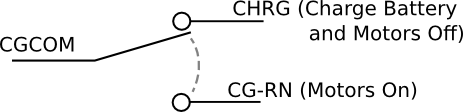
\includegraphics[scale=0.5]{chrg-run-switch}
\caption{The Charge/Run Switch}
\label{fig:chrgrun}
\end{figure}

\section{Programming Information}

\section{Trouble shooting}


\section{Glossery}
\begin{tabular}{| l | p{5cm}|}
\hline
SR Connector & Green 2-Way or 3-Way plug-in male connector with screw terminals. \\ \hline
Battery Connector & 2.1mm jack \\
\hline
\end{tabular}
\end {document}
